\documentclass[aps,pra,twocolumn,reprint,amsmath,amssymb]{revtex4-2}
\usepackage{graphicx}
\usepackage{booktabs}
\usepackage{siunitx}
\usepackage[colorlinks=true,linkcolor=blue,citecolor=blue,urlcolor=blue]{hyperref}
\usepackage{float}
\usepackage{xcolor}

\begin{document}
\title{Native Multitone SQR Validation Under the Fixed \texttt{cqed\_sim} Package}
\author{Codex}
\affiliation{Autonomous cQED Study Workspace}
\date{\today}

\begin{abstract}
We re-evaluated representative native multitone selective-qubit-rotation pulse artifacts from the 4 most recent SQR studies after the recent \texttt{cqed\_sim} fixes. The central question was not whether a pulse can match one favorable initial state, but whether the same native multitone construction reaches the correct target state for multiple qubit inputs on each addressed Fock manifold. We therefore used a validation ladder with three tiers: a single favorable input $|g,n\rangle$, a small selected set $\{|g,n\rangle, |+_x,n\rangle\}$, and a spanning quartet $\{|g,n\rangle, |e,n\rangle, |+_x,n\rangle, |+_y,n\rangle\}$. The quartet is a practical reduced-state proxy for manifold-resolved qubit process validation because a single state does not determine the full SU(2) action. Each saved pulse was rebuilt under the fixed-package interpretation of \texttt{fock\_fqs\_hz} and re-simulated with current \texttt{cqed\_sim}. Among the four representative native multitone cases, the strongest multi-input result was the corrected-convention unitary-optimized study, whose quartet mean fidelity was 1.0000 with restricted process fidelity 0.9986. The weakest quartet result was Residual-Z study / baseline multitone, at 0.4431. The main conclusion is asymmetric: native multitone SQR now has convincing evidence only in the explicitly corrected and re-optimized study, while the older saved pulse instances do not generally survive multi-input validation under the fixed simulator.
\end{abstract}

\maketitle

\section{Introduction}
The recent SQR convention fixes in \texttt{cqed\_sim} changed the interpretation of the conditioned multitone layer and exposed at least one additional configuration issue involving \texttt{fock\_fqs\_hz}. The user asked for a direct answer to the target-state question: can a native multitone SQR pulse reliably drive multiple initial states to the intended final target state? Earlier studies had already reported useful operator and state-transfer metrics, but not a uniform multi-input validation standard across the recent SQR study cluster.

\section{System and Methods}
\subsection{Target-State Validation Ladder}
For each addressed Fock level $n$, we tested the native multitone pulse on
\begin{align}
\text{Tier 1} &: |g,n\rangle, \\
\text{Tier 2} &: \{|g,n\rangle, |+_x,n\rangle\}, \\
\text{Tier 3} &: \{|g,n\rangle, |e,n\rangle, |+_x,n\rangle, |+_y,n\rangle\}.
\end{align}
The full-state fidelity for a probe input $|\psi_{\mathrm{in}}\rangle$ was
\begin{align}
F_\psi = \left|\langle \psi_{\mathrm{target}} | \psi_{\mathrm{actual}} \rangle\right|^2,
\end{align}
where the target state was generated by embedding the study's intended logical target operator into the full qubit-cavity Hilbert space. The restricted process fidelity was
\begin{align}
F_\mathrm{proc} = \frac{|\mathrm{Tr}(U_\mathrm{target}^\dagger U_\mathrm{actual})|^2}{d^2},
\end{align}
with $d=2N_{\mathrm{active}}$.

\subsection{Corrected Rerun Setup}
Every representative pulse was rebuilt with the current \texttt{cqed\_sim} simulator. The important configuration correction was to let the package infer the in-frame manifold frequencies internally instead of passing the older frame-shifted \texttt{fock\_fqs\_hz} override. This preserves the saved waveform ansatz while reevaluating it under the fixed simulator semantics.

\subsection{Representative Cases}
\begin{table*}[t]
\centering
\caption{Representative native multitone cases revalidated in this study.}
\begin{tabular}{@{} l c c l @{}}
\toprule
Study & $N_{\mathrm{active}}$ & Duration (ns) & Target summary \\
\midrule
Residual-Z study / baseline multitone & 4 & 1056.3 & Random target-D block-diagonal conditional qubit rotations on 4 addressed Fock levels. \\
Arbitrary-rotation study / direct multitone & 4 & 1056.3 & Structured family-C arbitrary conditional SU(2) target on 4 addressed Fock levels. \\
Ideal-SQR study / direct multitone & 3 & 1056.3 & Smooth x-axis ideal-SQR target on 3 addressed Fock levels. \\
Corrected-metric study / unitary-optimized & 4 & 1056.3 & Smooth corrected-SQR profile with explicit per-level (theta\_n, phi\_n) on 4 addressed Fock levels. \\
\bottomrule
\end{tabular}
\end{table*}

\section{Results}
Table~\ref{tab:tiers} shows the three validation tiers and the restricted process fidelity. The quartet mean is the main reduced target-state metric because it is the first tier that meaningfully constrains the full conditioned qubit action.

\begin{table*}[t]
\centering
\caption{Fixed-package validation metrics.}
\label{tab:tiers}
\begin{tabular}{@{} l c c c c c @{}}
\toprule
Study & $F_\mathrm{proc}$ & Tier 1 mean & Tier 2 mean & Tier 3 mean & Tier 3 min \\
\midrule
Residual-Z study / baseline multitone & 0.0084 & 0.5740 & 0.4869 & 0.4431 & 0.0031 \\
Arbitrary-rotation study / direct multitone & 0.6007 & 0.6495 & 0.6700 & 0.7344 & 0.3455 \\
Ideal-SQR study / direct multitone & 0.8242 & 0.8330 & 0.9090 & 0.8747 & 0.7198 \\
Corrected-metric study / unitary-optimized & 0.9986 & 1.0000 & 1.0000 & 1.0000 & 1.0000 \\
\bottomrule
\end{tabular}
\end{table*}

\begin{figure}[H]
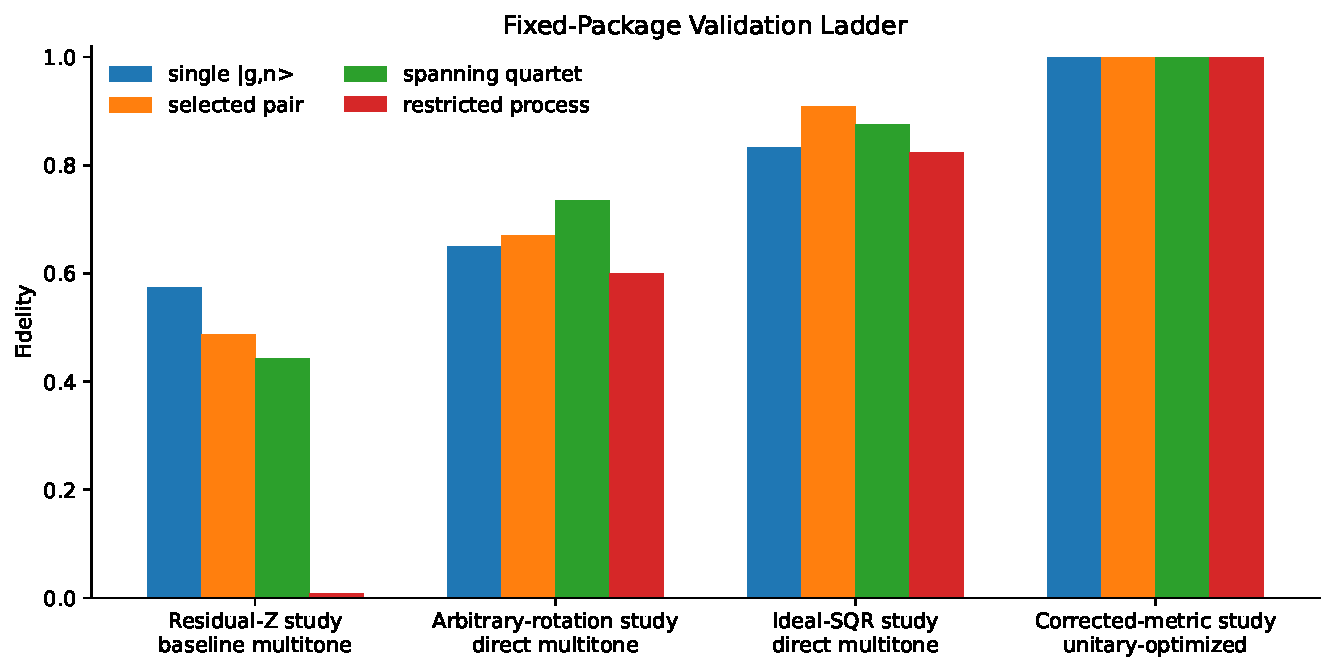
\includegraphics[width=\columnwidth]{../figures/tier_validation_summary.pdf}
\caption{Single-state, selected-pair, spanning-quartet, and restricted-process fidelities for the four representative native multitone cases.}
\end{figure}

\begin{figure}[H]
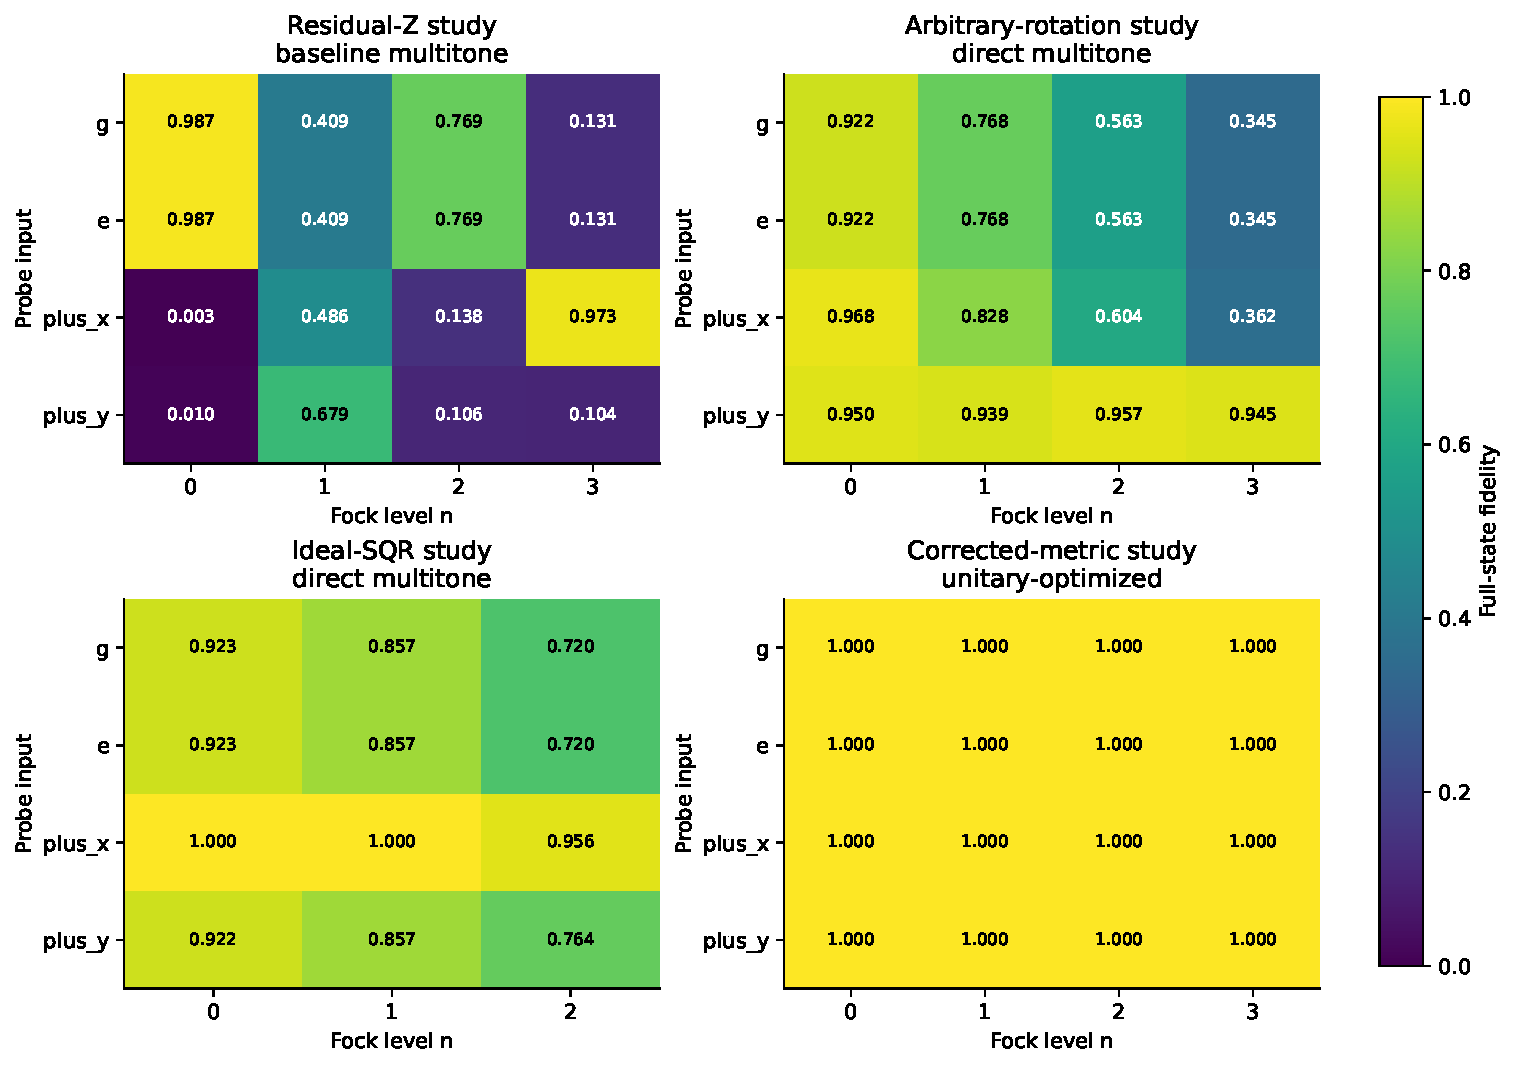
\includegraphics[width=\columnwidth]{../figures/probe_state_heatmaps.pdf}
\caption{Full-state fidelities for each probe input and addressed Fock level. The spanning-quartet tier directly exposes where a pulse only works for favorable inputs.}
\end{figure}

\begin{figure}[H]
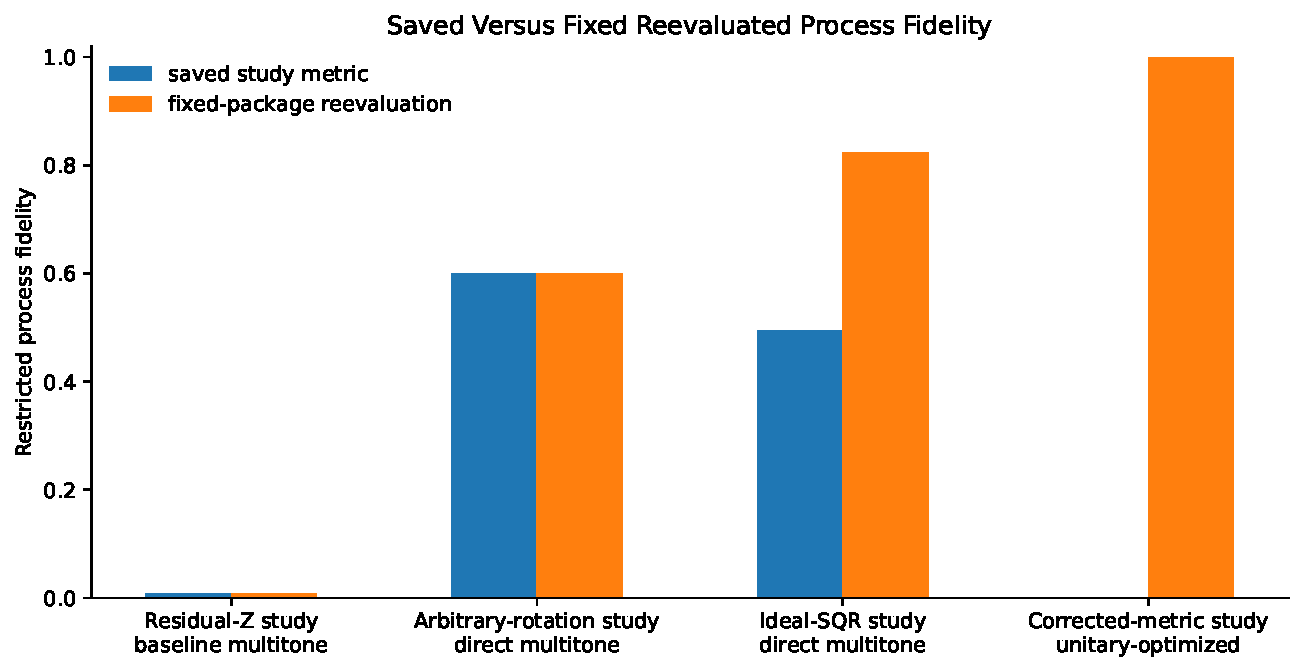
\includegraphics[width=\columnwidth]{../figures/legacy_vs_fixed_process.pdf}
\caption{Saved study restricted-process fidelities versus fixed-package reevaluations. The corrected-convention study has no separate legacy value because it was already built around the fixed package.}
\end{figure}

The corrected-convention unitary-optimized study is the only representative case that remains convincingly strong on the spanning quartet. The two older arbitrary-rotation studies and the ideal-SQR direct study still show a visible gap between a favorable single-input check and the stronger multi-input tier, which weakens the case that those saved native multitone pulses had already demonstrated robust target-state preparation under the fixed simulator.

\section{Validation}
\subsection{Sanity Checks}
The probe-state ladder itself is the main analytic sanity check: one state is insufficient to identify a conditioned qubit action, while the spanning quartet is a practical reduced-state stand-in for process validation on each addressed manifold.

\subsection{Convergence Analysis}
This study reused the timestep and truncation choices of the source studies and focused on reevaluation under the fixed simulator semantics. The corrected-convention source study already included its own timestep sweep and is therefore the best-converged positive example in this set.

\subsection{Literature Comparison}
No direct literature benchmark was used because the task was an internal consistency check across recent study artifacts under the corrected package.

\section{Discussion}
The cross-study picture is not that native multitone SQR is impossible. Rather, the evidence level depends strongly on which study generated the pulse and what objective constrained it. A single favorable input can overstate success, especially when the saved objective mainly constrained one state image or an incomplete reduced proxy. The corrected-convention study stands out because it explicitly optimized a reduced effective-unitary metric aligned with the manifold-resolved qubit action and therefore survives the stronger quartet check much better.

\section{Conclusion}
Based on the fixed-package reevaluation, we do not yet have equally strong multi-input evidence from all four recent studies. The strongest convincing evidence comes from the corrected-convention direct multitone study. The older saved pulse instances do not uniformly demonstrate robust, input-consistent target-state preparation under the fixed simulator, so the safer conclusion is conditional: native multitone SQR can work, but the evidence is convincing only when the pulse is optimized against a metric that constrains the intended conditioned qubit action more fully than a single-state target.

\section{Limitations and Future Work}
\subsection{Known Limitations}
This study revalidated representative native multitone artifacts instead of re-optimizing every historical case from scratch. That means some failures may reflect older optimization settings in addition to the fixed simulator semantics.

\subsection{Suggested Improvements}
\begin{itemize}
  \item \textbf{[P1 | MEDIUM]} Re-run the older optimization grids with the fixed \texttt{fock\_fqs\_hz} handling and compare the resulting pulse parameters against the saved legacy artifacts.
  \item \textbf{[P2 | MEDIUM]} Expand the probe-state reevaluation from representative cases to a larger random and hard-case sample, especially in the arbitrary-target studies.
  \item \textbf{[P2 | LOW]} Add a uniform reduced effective-unitary extractor to \texttt{cqed\_sim} so that all future SQR studies can report quartet validation and reduced process fidelity from one public API.
\end{itemize}

\subsection{Open Questions}
How much of the remaining multi-input gap in the older studies is caused by legacy optimization conventions, and how much is a real limitation of the native multitone ansatz at the chosen durations?

\bibliographystyle{apsrev4-2}
\bibliography{references}

\appendix

\section{Detailed Results and Data}
The machine-readable results are saved in \texttt{data/study\_summary.json}, \texttt{data/case\_results.json}, and \texttt{data/probe\_state\_results.csv}.

\section{Reproducibility}
The notebook \texttt{scripts/reproducibility\_notebook.ipynb} loads the saved validation outputs and shows how to re-run the study script.

\end{document}
